% ****** Start of file aipsamp.tex ******
%
%   This file is part of the AIP files in the AIP distribution for REVTeX 4.
%   Version 4.1 of REVTeX, October 2009
%
%   Copyright (c) 2009 American Institute of Physics.
%
%   See the AIP README file for restrictions and more information.
%
% TeX'ing this file requires that you have AMS-LaTeX 2.0 installed
% as well as the rest of the prerequisites for REVTeX 4.1
%
% It also requires running BibTeX. The commands are as follows:
%
%  1)  latex  aipsamp
%  2)  bibtex aipsamp
%  3)  latex  aipsamp
%  4)  latex  aipsamp
%
% Use this file as a source of example code for your aip document.
% Use the file aiptemplate.tex as a template for your document.
\documentclass[%
 aip,
%jmp,%
%bmf,%
%sd,%
rsi,%
 amsmath,amssymb,
%preprint,%
 reprint,%
%author-year,%
%author-numerical,%
]{revtex4-1}

\usepackage{graphicx}% Include figure files
\usepackage{dcolumn}% Align table columns on decimal point
\usepackage{bm}% bold math
%\usepackage[mathlines]{lineno}% Enable numbering of text and display math
%\linenumbers\relax % Commence numbering lines

\newcommand	 {\sbar}	{{s}}
\newcommand	 {\rbar}	{{r}}
\newcommand	 {\hi}		{{h_\mathrm{i}}}
\newcommand	 {\pii}  	{{p_\mathrm{i}}}
\newcommand	 {\kb}		{{k_\mathrm{B}}}
\newcommand	 {\Tlow}	{{T_\mathrm{low}}}
\newcommand 	 {\Pnat} 	{{P_\mathrm{nat}}}
\newcommand {\QIA}	{{Q_\mathrm{IA}}}
\newcommand {\QIB}	{{Q_\mathrm{IB}}}
\newcommand {\QIIA}	{{Q_\mathrm{IIA}}}
\newcommand {\QIIB}	{{Q_\mathrm{IIB}}}
\newcommand {\Pcut}     	{{P_\mathrm{cut}}}
\newcommand {\TlowI}     {{T^\mathrm{I}_\mathrm{low}}}
\newcommand {\TlowII}    {{T^\mathrm{II}_\mathrm{low}}}
\newcommand {\Ptot}	{{P_\mathrm{tot}}}
\newcommand {\PIA}    	{{P_\mathrm{IA}}}
\newcommand {\PIB}    	{{P_\mathrm{IB}}}
\newcommand {\PIIA}    	{{P_\mathrm{IIA}}}
\newcommand {\PIIB}    	{{P_\mathrm{IIB}}}
\newcommand {\Eave}	{{E_\mathrm{ave}}}
\newcommand {\sigE}	{{\sigma_{\left < E \right >}}}
\newcommand {\SR}		{${\mathrm{S16}_{144}}$}
\newcommand {\SI}		{${\mathrm{S16}_{1024}}$}	
\newcommand {\SII}		{${\mathrm{S16}_{1024}}$}

\begin{document}

\preprint{AIP/123-QED}

\title[Multisequence Monte Carlo simulations]{Multisequence algorithm for coarse-grained biomolecular simulations: application to protein fold switching}

\author{A. Aina}
\author{S. Wallin}
\email{swallin@mun.ca}
\affiliation{ 
Memorial University of Newfoundland, Department of Physics and Physical Oceanography, A1B 3X7 St John's, NL, Canada}

\date{\today}

\begin{abstract}
We consider a generalized-ensemble algorithm for coarse-grained simulations of biomolecules, which allows the thermodynamic behaviors of two or more sequences to be determined in a single multisequence run. By carrying out a random walk in sequence space, the method also enhances conformational sampling. Escape from local energy minima is accelerated by visiting sequences for which the minima are more shallow or absent. We apply the method to an intermediate-resolution coarse-grained model for protein folding with 7 atoms per amino acids. The potential for large-scale coverage of sequence space is explored by applying the method to two sets with $>$1,000 sequences each. The resulting thermodynamic data is used to explore the sequence-structure and sequence-stability relationships between pairs of protein folds with different secondary structures. The potential implications for the evolution of new protein folds are discussed. 
 
\end{abstract}

\pacs{Add  here}
                             
\keywords{Generalized ensembles, simulated tempering, protein folding, coarse-graining, evolution}


\maketitle

\section{Introduction}
\noindent
Modern investigations into biophysical properties of biomolecular systems are routinely carried out not only on a single species but on multiple molecular variants.~\cite{Vukmirovic2000,Nickson2010} For example, protein engineering methods are used to provide mechanistic insight into the specificity of protein-protein and protein-DNA interactions, to compare the  conformational propensities of disease-related mutations of aggregation-prone proteins, and optimize biomolecular properties through directed evolution. Moreover, large-scale screening techniques such as phage display and microarray chips are used to provide biophysical properties across entire genomes. In short, through the study of a biomolecular system and related variants molecular variants are studied in order to gain a more complete picture of the biophysical and biochemical properties of the system and provide evolutionary context. 

While protein or DNA sequences are easily changed on the computer, the high computational cost of simulating even a single moderately-sized biomolecule makes systematic explorations of sequence space challenging. Some notable efforts have nonetheless been attempted, including simulations of all 136 unique tetranucleotide sequences in B-DNA oligonucleotides using all-atom explicit water molecular dynamics.~\cite{Beveridge2004}

Here we explore a Monte Carlo (MC)-based algorithm for calculating the folding thermodynamics of multiple protein sequences in a single enhanced run. The algorithm relies on sampling at fixed temperature a generalized ensemble in which the sequence is treated as a dynamic parameter. Hence, this multisequence MC method includes two main types of updates: conformational updates $\rbar\rightarrow\rbar'$ and sequences updates $\sbar\rightarrow\sbar'$. As illustrated in Fig.~1, this approach requires that $\rbar$ and $\sbar$ are ``perpendicular" coordinates such that the potential energy of the model can be written in terms of two independent variables, $E(\sbar,\rbar)$. While this may be hard to achieve for detailed protein models, it is likely possible for many coarse-grained models. 

We first apply the MS algorithm to a set of 144 model sequences with 16 amino acids and compare with the simulated tempering (ST) algorithm. We find that the computational efficiency of the MS algorithm is never less efficient than ST even at the lowest studied temperature. The model folds spontaneously designed sequences into stable native states with diverse protein-like sequences, and captures features such as mutational robustness. It therefore provide a biophysical basis for the sequence-structure and sequence-stability relationships of proteins at a conceptual level. This model has been used, e.g., to study the sequence-structure relationship of proteins in the "marshlands" between protein folds. Experimental studies have indicated that single point mutations are capable to take change one protein fold into another. The multisequence algorithm allow us to characterize the stability of and structure of all 1,024 sequence in the binary space between the two folds. The implication of these results for the fold switching and evolution is discussed. \\

We then demonstrate that the multisequence algorithm can be used to calculate the thermodynamic behavior for $>1,000$ sequences in a 3-letter model for protein folding~\cite{Bhattacherjee2012} at temperatures well below the typical folding temperatures $T_\mathrm{f}$ of the included sequences.  

While the 16-amino acid A1 and N1 sequences fold into $\alpha$-helical and $\beta$-hairpin folds, respectively, the two 35-amino acid sequences A2 and TA adopt the folds denoted IIA and IIB, as shown in Fig.~X. 

The large number of sequences considered allows us to carry out a much more systematic analysis than previously~\cite{Holzgrafe2014,Holzgrafe2015} of the sequence-structure-stability relationship in the sequence region that connect these two folds pairs. We find that...


\begin{figure}
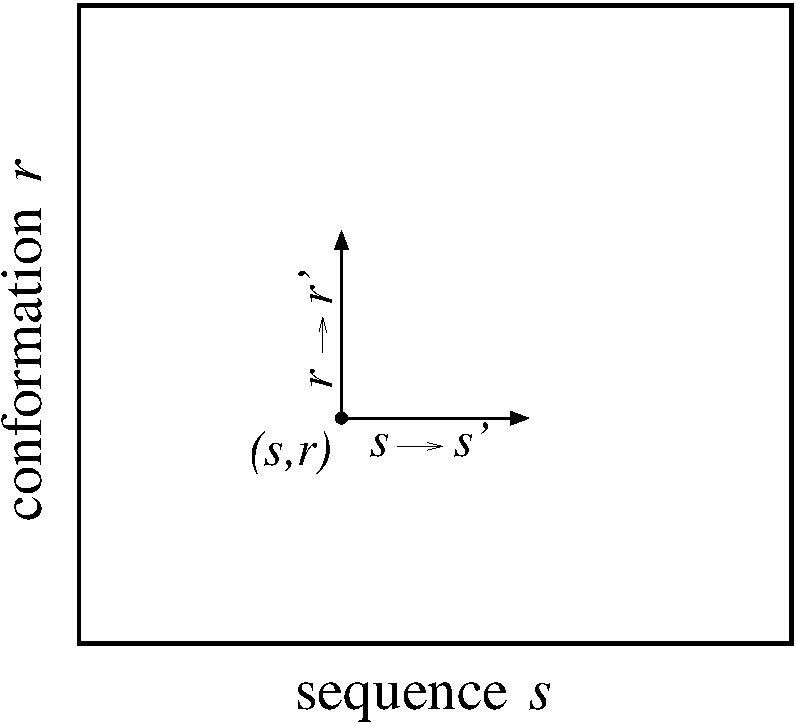
\includegraphics[width=4.2cm]{Fig1}
\caption{The two types of Monte Carlo updates in the multisequence Monte Carlo algorithm.}
\end{figure}

\section{Theory}

\subsection{Generalized-ensemble algorithms and simulated tempering}
\noindent
Conventional Monte Carlo simulations of the canonical distribution is problematic at low temperatures $T$ for many physical systems because simulations tend to become trapped in local energy energy minima and hamper representative sampling of configurational space. The basic idea of generalized-ensemble algorithms~\cite{Mitsutake2001} is to alleviate this trapping problem by sampling states using a non-Boltzmann weight factor and/or expand the state space with additional dynamical parameters, such that a more efficient random walk in potential energy can be achieved. 

A well-known generalized-ensemble algorithm is simulated tempering (ST),~\cite{Marinari1992,Lyubartsev1992} in which it is the temperature $T$ that becomes a dynamic parameter. In this scheme, frequent visits to high-$T$ allow simulations to readily escape from local energy traps. The ST algorithm thus simulates the joint probability distribution 
\begin{equation}
P(\rbar,m) =\dfrac{1}{\hat{Z}} e^{-\beta_m E(\rbar) + g_m}\,,
\label{ST}
\end{equation}
where  $\beta_m=1/k_\mathrm{B} T_m$, $\{T_m\}_{m=1}^\mathrm{M}$ a set of temperatures and $k_\mathrm{B}$ is Boltzmann's constant. The normalization constant in Eq.~\ref{ST} is  
\begin{equation}
\hat{Z} = \sum_r \sum_{m=1}^{\mathrm{M}}e^{-\beta_m E(\rbar) + g_m}\,,
\end{equation}
where the first sum is over all conformations $\rbar$. The simulation parameters $g_m$ control the marginal probability distribution
\begin{equation}
P(k) = \frac{1}{\hat{Z}}\sum_r e^{-\beta_m E(\rbar) + g_m} \,,
\end{equation}
and must therefore be carefully chosen. A common and convenient choice is $g_m\approx \beta_m F_m$, where $F_m$ is the free energy at temperature $T_m$. With this choice, $P(k)$ becomes approximately flat ensuring all temperatures are frequently visited. 

\subsection{Multisequence algorithm}
\noindent 
The basic idea of the MS algorithm for biomolecular simulation is to let the sequence $\sbar$ become a dynamic parameter rather than the temperature as in ST. A dynamic $\sbar$ is technically feasible as long as the potential energy can be written as $E(\sbar,\rbar)$, where $\sbar$ and $\rbar$ are independent variables. This is the case in our coarse-grained protein model with only backbone degrees of freedom and can also be achieved for more detailed  models~\cite{Bhattacherjee2013,Wallin2017}. 

In analogy with ST, the MS algorithm simulates the joint probability distribution
\begin{equation}
P(\sbar,\rbar) =\dfrac{1}{\tilde{Z}}e^{-\beta E(\sbar,\rbar) + h(\sbar)}\,, 
\label{MS}
\end{equation}
where  
\begin{equation}
\tilde{Z} = \sum_{\sbar}\sum_{\rbar} e^{-\beta E(\sbar,\rbar)+ h(\sbar)}\,
\end{equation}
and the first sum goes over a set of allowed sequences $\sbar$. The simulation parameters $h(\sbar)$, similarly to the parameters $g_m$ in ST, control the marginal distribution $P(\sbar)=\tilde{Z}^{-1}\sum_{\rbar} e^{-\beta E(\sbar,\rbar)+ h(\sbar)} = \tilde{Z}^{-1}e^{-\beta F(\sbar)+ h(\sbar)}$ and a roughly flat $P(\sbar)$ can be achieved by choosing $h(\sbar) \approx \beta F(\sbar)$, where $F(\sbar)$ is the free energy of sequence $\sbar$ at temperature $T$. 

Two types of MC updates are required to sample from the distrubution in Eq.~\ref{MS}, ordinary conformational update $\rbar\rightarrow\rbar'$ and mutational updates $\sbar\rightarrow\sbar'$. The acceptance probabilities for the latter  becomes
\begin{equation}
P_\mathrm{acc} (\sbar\rightarrow\sbar') = \min [1, \exp\{-\beta\Delta E+\Delta h\}]\,,
\label{accrej}
\end{equation}
where $\Delta E = E(\sbar',\rbar)-E(\sbar,\rbar)$ and $\Delta h = h({\sbar'})-h(\sbar)$.

\section{Model and Methods}
\subsection{Coarse-grained 3-letter model for protein folding}
\noindent
All calculations were carried out using the coarse-grained model for protein folding developed in Ref.~\citenum{Bhattacherjee2012}. In this model, there are 3 different amino acid types: hydrophobic (h), polar (p) and turn-type (t). The backbone chain is represented atomistically by the N, H, $\mathrm{C}_\alpha$, $\mathrm{H}_{\alpha 1}$, C$'$ and O atoms. By contrast, the sidechain represention is simplified to a single enlarged $\mathrm{C}_\beta$ atom, which is geometrically identical for h and p types. The sidechain is absent for the t type which instead has an $\mathrm{H}_{\alpha 2}$ atom. The t type is therefore closely related to glycine. All bond lengths, bond angles, and peptide plane angles (180$^\circ$) are held fixed. Hence, an $N$-amino acid chain conformation $\rbar$ can, for any sequence $\sbar$, is therefore described by the set of 2$N$ backbone torsional angles $\{\phi_i$, $\psi_i\}_{i=1}^{N}$. 
 
This geometrical description is paired with a simplified but finely tuned energy function with 4 terms: $E= E_\mathrm{ev} + E_\mathrm{loc} + E_\mathrm{hb} + E_\mathrm{hp}$. The first two, $E_\mathrm{ev}$ and $E_\mathrm{loc}$, represent excluded-volume effects of all atoms and local electrostatic effects, respectively. The hydrogen-bond energy, $E_\mathrm{hb}$, represents directionally dependent interactions between NH and CO groups which are necessary for secondary structure formation. Finally, the ``hydrophobicity" term, $E_\mathrm{hp}$, implements pairwise Lennard-Jones-like interactions between the $C_\beta$ atoms of h amino acids which are necessary for driving chain collapse during folding. Various model parameters, e.g., the strengths of hydrophobic attractions and hydrogen bonding, were determined based on the ability of the model to spontaneously fold a set of model sequences with 18-54 amino acids into  structurally diverse and thermodynamically stable native states with both $\beta$ and $\alpha$-structure. As it turned out, this strategy made the model robust enough to fold sequences designed to have mised $\alpha$ and $\beta$ structure. 

\subsection{Model sequences}

The sequences studied in this work are summarized in Table~I. 
 
\begin{table}
\caption{\label{tab1} List of model sequences of different lengths $N$ studied in this work.}
\begin{ruledtabular}
\begin{tabular}{lcr}
Name & $N$ & Sequence\footnote{In addition, we study two sets of 1,024 sequences derived from the A1-N1 and A2-TN pairs (see text) denoted $\mathrm{S16}_{1024}$  and $\mathrm{S35}_{1024}$, respectively, and a restricted set $\mathrm{S16}_{144}$ with 144 sequences taken from S16 ($\mathrm{S16}_{144}$ was also studied in Ref.~\protect\citenum{Holzgrafe2014}). } \\
\hline
A1 & 16 & pphpphhpphpphhpp \\
N1 & 16 & phphphpttphphphp \\
R1 & 16 & \textbf{(add)}\\
R2 & 16 &  \textbf{(add)}\\
A2 & 35 & (A1)ttt(A1)\\
TN & 35 & (A1)ttt(N1)\\
\end{tabular}
\end{ruledtabular}
\end{table}


\subsection{Monte Carlo simulation parameters}
\noindent
Both ST and MS simulations are carried out with two types of conformational updates $\rbar\rightarrow\rbar'$: (1) a global pivot move (20\%) which randomly picks a $\phi_\mathrm{i}$ angle or $\psi_\mathrm{i}$ angle and assigned a new value between $-\pi$ and $\pi$; and (2) a semi-local move (80\%) which turns the $\phi_\mathrm{i}$ and $\psi_\mathrm{i}$-angles of 4 consecutive amino acids in a coordinated manner.~\cite{Favrin2001} In MS simulations, sequence updates $\sbar\rightarrow\sbar'$ are carried out by randomly picking a new sequence $\sbar'\ne\sbar$ and applying the accept-reject criterion in Eq.~\ref{accrej}. A sequence move is attempted every $1,000$ MC step while temperature updates $m\rightarrow m'$ are attempted every 100 steps. The simulations carried out in this work are summarized in Tables~II.

\begin{table}
\caption{\label{tab2} List of simulations carried out in this work. }
\begin{ruledtabular}
\begin{tabular}{lccccr}
Runs & Algorithm & $\kb T$  & MC steps &  Sequences\\
\hline
32 & ST & 0.43--0.65 & $8\times 10^6$ &A1\\ 
32 & ST & 0.43--0.65 & $8\times 10^6$ &N1\\ 
32 & ST & 0.43--0.65 & $8\times 10^6$ &R1\\ 
32 & ST & 0.43--0.65 & $8\times 10^6$ &R2\\ 
32$\times$8\footnote{32  runs per temperature for 8 temperatures in the range given.} & MS &0.43--0.65& $144\times 10^6$ & $\mathrm{S16}_{144}$\\
16 & MS & 0.43  & $5\times 10^9$ &  $\mathrm{S16}_{1024}$ \\
16 & MS & 0.46 & $4\times 10^9$ &  $\mathrm{S35}_{1024}$ \\
\end{tabular}
\end{ruledtabular}
\end{table}

\subsection{Observables}
\noindent
Fold stabilities are calculated as in Ref.~\citenum{Holzgrafe2015} and also described briefly below. We define first two structural similarity measures $\QIA$ and $\QIB$ for folds IA and IB, respectively, indicating what fraction of the fold-specific backbone-backbone hydrogen bonds have been formed. The fold IA-hydrogen bonds are (2,6), (3,7), (4,8), (5,9), (6,10), (7,11), (8,12), (9,13), (10,14), (11,15) and the fold IB-bonds are (3,14), (5,12), (7,10), (10,7), (12,5), (14,3), where (i,j) indicates a hydrogen bond between the CO group of amino acid i and the NH group of amino acid j. The  stabilities of fold IA and IB are then defined as the probabilities $\PIA = P(\QIA\ge0.8)$ and $\PIB = P(\QIB\ge0.80)$, respectively, i.e., stability is the probability that at least 80\% of the fold's hydrogen bonds are formed. $\PIA$ and $\PIB$ depend on both sequence $\sbar$ and temperature $T$. For example, $\PIA=0.xx$ for A1 and $\PIB=0.xx$ for N1 at $\kb T = 0.43$. Structural similarity measures for 35-amino acid folds IIA and IIB are defined as $\QIIA = ( Q_\mathrm{IA}^\mathrm{1-16} + Q_\mathrm{IA}^\mathrm{20-35} + Q_\mathrm{tert}) ) / 3$ and $\QIIB = ( Q_\mathrm{IA}^\mathrm{1-16} + Q_\mathrm{IB}^\mathrm{20-35} + Q_\mathrm{tert} ) / 3$, respectively, where superscripts on $\QIA$ and $\QIB$ indicate over which amino acid positions those measures are applied to within the longer 35 amino acid sequences and $Q_\mathrm{tert}$ is a measure that counts the number of $C_\beta$-$C_\beta$ contacts between the two secondary structure elements of these folds.~\cite{Holzgrafe2015} As for IA and IB, the stabilities of folds IIA and IIB are defined as $\PIIA = P(\QIIA\ge0.8)$ and $\PIIB = P(\QIIB\ge0.80)$, respectively. 
%In calculating $Q$ values, a hydrogen bon�d is considered formed if (i) the NHO and COH angles are both $>90^\circ$ and (ii) the HO distance is $<2.7$~{\AA}. 

\begin{figure}
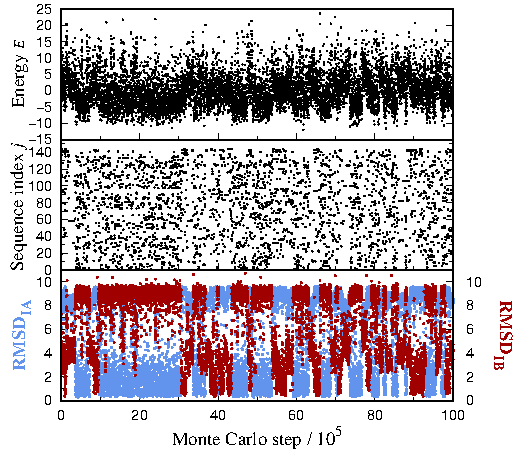
\includegraphics[width=6.0cm]{MCtraj}
\caption{(A) Example simulation trajectory of the MS algorithm applied to the sequence set $\mathrm{S16}_{144}$. The plot shows the MC evolution of the sequence $\sbar$ (numbered 1--144), the total potential energy $E$ and the root-mean-square deviation (RMSD) calculated against the fold IA (light blue) and fold IB (dark red) structures shown in (B). The simulation is carried out at $\kb T = 0.43$ corresponding to the lowest studied temperature.  (B) Representative structures of fold IA and fold IB, selected to be the minimum-energy conformations found for the sequences A1 and N1, respectively. (C) Representative fold IIA and fold IIB structures selected to be the minimum-energy conformations of A2 and TN, respectively. }
\end{figure}

%
%\begin{equation}
%Q_\mathrm{\alpha\beta\beta} = ( Q_\alpha^\mathrm{1-12} + Q_\beta^\mathrm{XX} +Q_\beta^\mathrm{20-35} + Q_\mathrm{tert} ) / 4
%\end{equation}
%
%
%\begin{equation}
%Q^*_\mathrm{\alpha\beta} = [ \max(Q_\alpha^\mathrm{1-16},Q_\beta^\mathrm{XX}) +Q_\beta^\mathrm{20-35} + Q_\mathrm{tert}) ] / 3
%\end{equation}
%

\section{Results}

\subsection{Computational efficiency of the multisequence algorithm}
\noindent
To assess the computational efficiency and properties of the multisequence algorithm, we used as a test case the set of 144 3-letter model sequences with 16 amino acids studied in Refs.\cite{Holzgrafe2014} Two of the sequences are A1 and N1 which were designed to fold into stable $\alpha$-helix and $\beta$-hairpin structures, respectively. A1 and N1 differ at 10 positions such that 10 consecutive point mutations can transform A1 into N1, and vice versa. The binary sequence space between A1 and N1 in which any combination of these mutations have been carried out, therefore contains $2^{10}=1,024$ sequences. The 144 sequences were selected from this binary space with the constraint that the total number of h-amino acids are not too high or too unevenly distributed.~\cite{Holzgrafe2014}

\begin{figure}
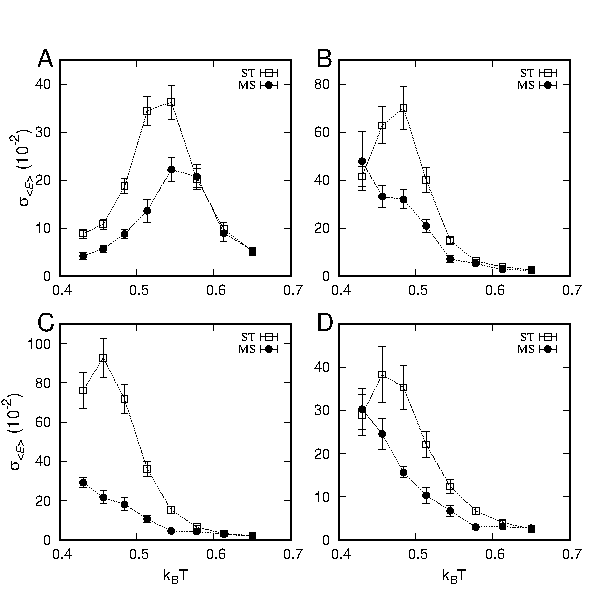
\includegraphics[width=8.0cm]{Stderr}
\caption{Computational efficiency of the multisequence and simulated tempering algorithm.}
\end{figure}


We apply the multisequence algorithm to this set of 144 sequences across a range of temperatures. Figure~2 illustrates a typical simulation carried out at the lowest temperature, $\Tlow$, which is well below the folding temperature of both A1 and N1~\cite{Holzgrafe2014,Holzgrafe2015}. From the MC evolution of the total energy $E$, sequence index j, and similarity measures $Q_A$ and $Q_B$, it is evident that visits to various sequences drive transitions into a range of structural states. For example, visits to A1 ($\mathrm{j}=1$) and N1 ($\mathrm{j}=144$) tend to coincide with visits to high-$Q_A$ and high-$Q_B$ conformations, respectively, as is necessary to generate the correct conformational ensembles for these sequences.

Sequence updates $\sbar\rightarrow\sbar'$ are carried out by picking a new sequence $\sbar'$ randomly from the entire set of allowed sequences. Therefore, a sequence update typically changes more than one amino acid position. In other words, if the step size in sequence space is $\Delta H$, then typically $\Delta H>1$. Interestingly, despite the large $\Delta H$ and low $T$, the overall (average) acceptance rate $P_\mathrm{acc}=0.xx$ for $\sbar\rightarrow\sbar'$ updates which is not unreasonably low. Higher $P_\mathrm{acc}$ can be obtained by restricting proposed moves such that $\Delta H\le\Delta H_\mathrm{max}$, as shown in Figure~3. For example, an acceptance rate close to the oft-quoted rule-of-thumb value $0.25~\cite{Gilks1996} $ is obtained with $\Delta H_\mathrm{max}=4$, and with $\Delta H_\mathrm{max} = 1$ (only point mutations), $P_\mathrm{acc}=0.xx$. For simplicity, in this work, all simulations are carried without restrictions on how new sequences $\sbar'$ are drawn. 

\begin{figure}
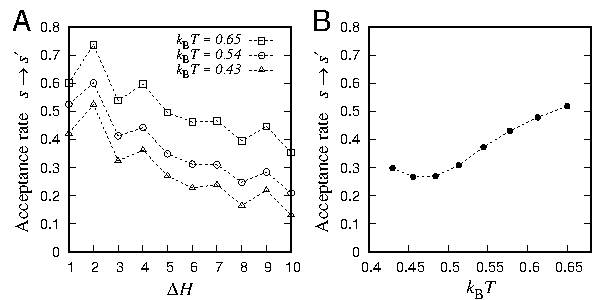
\includegraphics[width=7.8cm]{Pacc}
\caption{Acceptance rates for $\sbar\rightarrow\sbar'$ updates in MS simulations of the {\SR} sequence set as a function of (A) the number of changed amino acid positions  and (B) temperature. }
\end{figure}

To assess computational efficiency, we compare with results from simulated tempering (ST) simulations carried out on 4 of the 144 sequences, namely A1 and N1 and the two sequences R1 and R2 chosen randomly at $H=4$ and $H=6$ from A1, respectively (see Table~1). While ST provides the thermodynamics of a given sequence across the 8 temperatures $T_1, ..., T_8$ in a single run, a single MS simulation provides the thermodynamics of all 144 sequences for one $T_\mathrm{i}$. We adjust the simulation lengths for ST and MS runs such that an identical number of sampled conformations are obtained for each $\sbar$ and $T_\mathrm{i}$ combination, ensuring also that similar computational resources are used for the two algorithms. 

Figure 4 shows the statistical error, $\sigE$, estimated for the average energy, $\left <E\right >$, for the 4 different sequences. 

\begin{figure*}
\rotatebox{0}{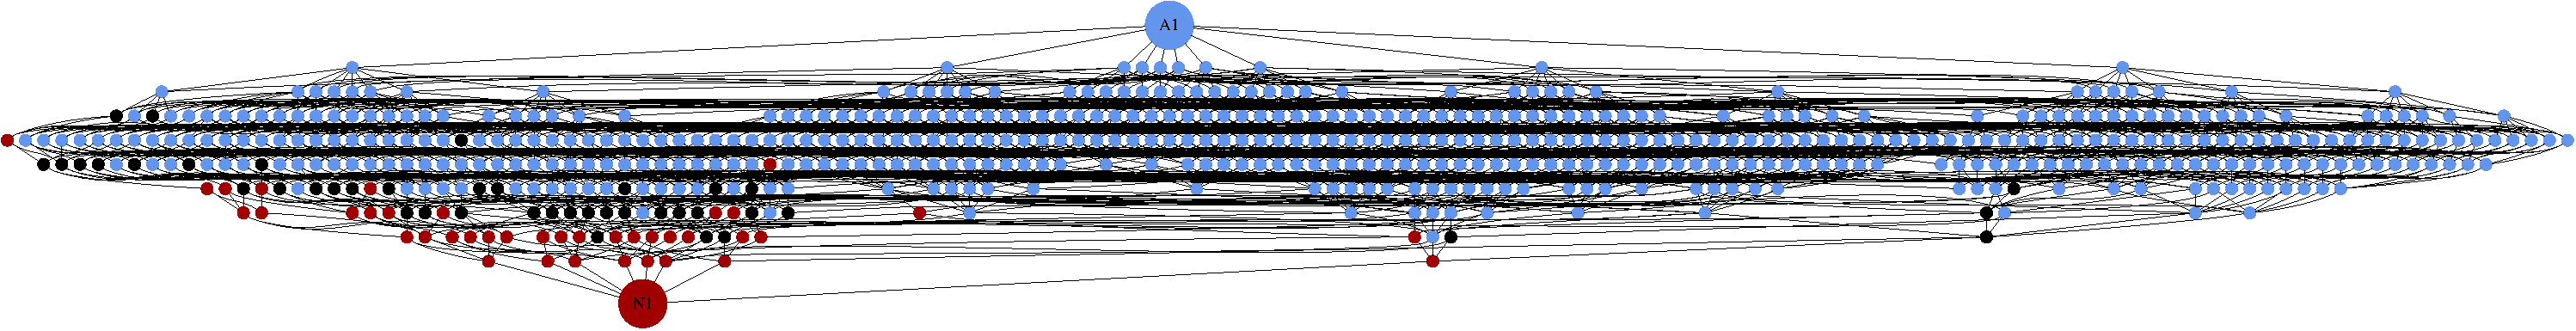
\includegraphics[width=16.6cm]{ntwk16}}\\
\rotatebox{0}{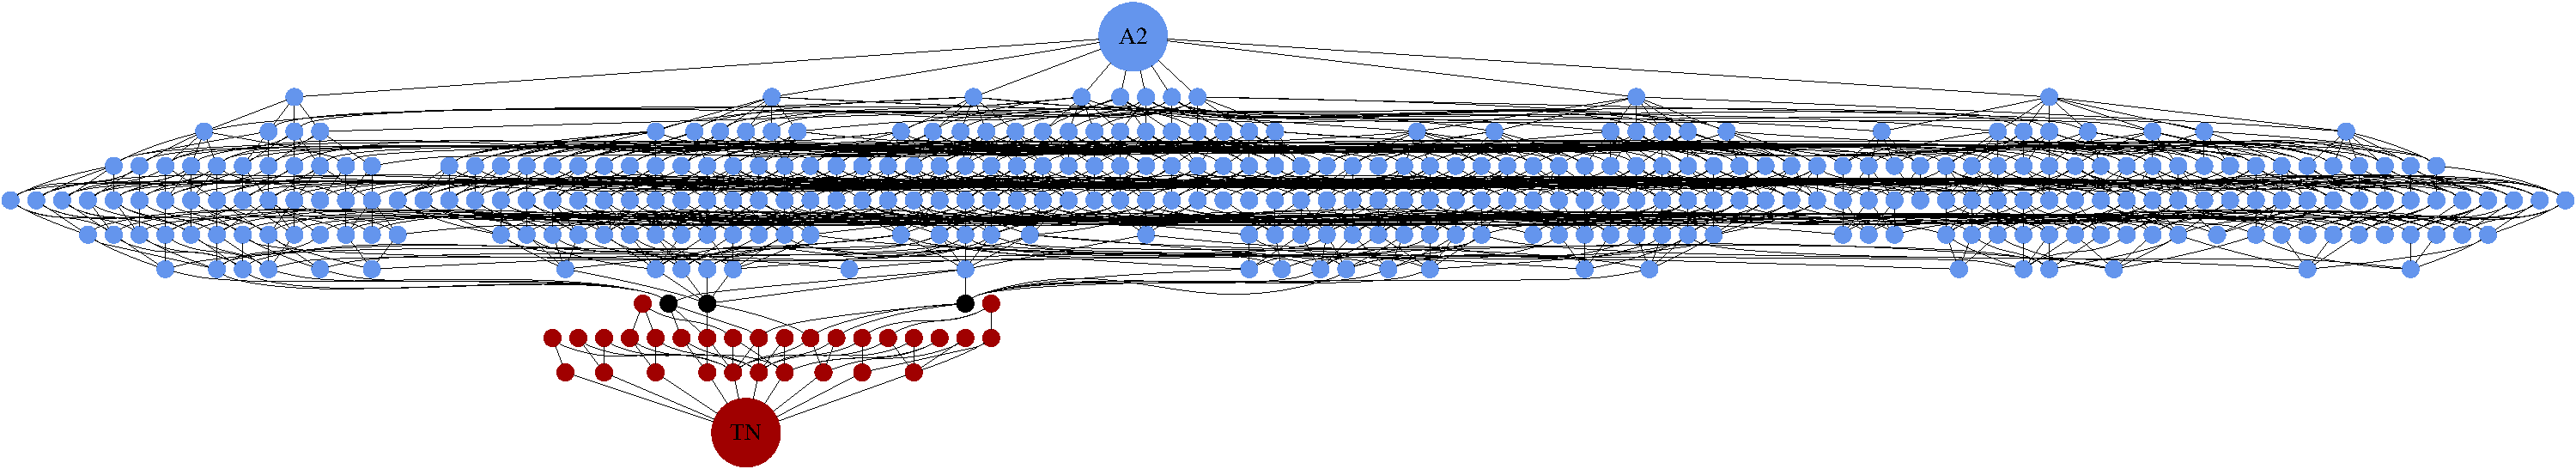
\includegraphics[width=12.6cm]{ntwk35}}
\caption{Networks of the A1-N1 (top) and A2-TN (bottom) binary sequence space. }
\end{figure*}

Hence, we conclude that in the comparison made above the computational efficiency of the MS algorithm is comparable to ST. It must be stressed, however, that while the ST simulation requires that the thermodynamic behavior is calculated at a range of temperatures, MS works well on its own directly at low temperatures. ST was introduced as an extension to the standard, fixed-$T$ Metropolis-Hastings algorithm in order to overcome the poor mixing of states at low temperatures, i.e., the tendency for the simulations at low $T$ to become trapped in local free energy minima. The MS algorithm, however, efficiently calculates the thermodynamics at low $T$'s without visits to other $T$'s. In the MS algorithm, it is visits to sequences with poor native state stability rather than high $T$'s that drive the decorrelation of generated states and escape from local traps. This way, calculation of low-$T$ thermodynamics is enhanced in MS simulations while at the same time enhancing coverage in sequence space. This makes the MS algorithm ideal for situations in which the finite-$T$ thermodynamic behavior of multiple sequences are of interest. 

\vspace{12pt}
\subsection{A1-N1 and A2-TN binary sequence spaces}
\noindent
We now apply the MS algorithm to the sets {\SI} and {\SII} which represent the full binary sequence spaces for the A1-N1 and A2-TN systems, respectively. Both sets include $2^{10}=1,024$ sequences. Using MS simulations, we determined the thermodynamic behavior at the temperatures $\TlowI$ and $\TlowII$ for the A1-N1 and A2-TN systems, respectively (see Table~1). In particular, this allow us to find the stabilities of folds IA and IB ($\PIA$ and $\PIA$) for all sequences in {\SI} and the stabilities of folds IIA and IIB ($\PIIA$ and $\PIIB$) for all sequences in {\SII}.


Having calculated these fold stabilities, we are in a position to determine if there are pathways in sequence space that lead to IA-IB or IIA-IIB fold changes without passing through an unstable intermediate sequence. To this end, we construct graphs in which each stable sequence is represented by a node and any two nodes are connected if their sequences differ at only one amino acid position. To determine if a sequence is stable we used the criterion $P_\mathrm{tot}>\Pcut$, where  $\Ptot = \PIA + \PIB$ and $\PIIA + \PIIB$ for A1-N1 and A2-AN1, respectively. The precise network obtained depends, of course, on the cut-off value of $\Pcut$. In general, a higher $\Pcut$ means a selection of more stable pathways. Fig.~5 shows the networks obtained with $\Pcut=0.50$. The number of viable mutational pathways that connect the start and end points are 516,972 between A1 and N1 and  57,912 between A2 and AN1. Because there are $10! =3,628,800$ possible mutational pathways between start and end points in both cases, these pathways represent 14.2 \% and 1.6 \% of all possible pathways in A1-N1 and A2-AN1, respectively. Hence, A1 and N1 are rather highly connected at this stability threshold. For $\Pcut=0.60$, the numbers are 104,640 pathways (2.9\%) for A1-N1 and 22,512 (0.6\%) pathways for A2-AN1. We find that there are no possible A1-to-N1 or A2-to-AN1 pathways when $\Pcut\ge0.74$ and $\Pcut\ge 0.66$, respectively. \\

\subsection{Stability properties of fold-to-fold mutational pathways}
\noindent 
An apparently general characteristic of designed and natural protein folding switching is that the stability of sequences near the switch point have reduced stability.~\cite{Bryan2010} The results from our model exhibit a similar trend. Fig.~6A and B shows the total stability $\Ptot$ at different mutational distances between start and end points. Intermediate sequences are less stable than at distances $h=0$ and $h=10$, although there are large variations as indicated by the spread between upper and lower bounds. Nonetheless, there is a clear statistical trend that sequences become gradually less stable as successive mutations are applied to any of the 4 starting points until a minimum is reached. 
%These minima in stability occur closer to N1 and TN in the two systems, respectively, indicating that the IA/IIA folds are more mutationally robust than the IB/IIB folds. 

\begin{figure}
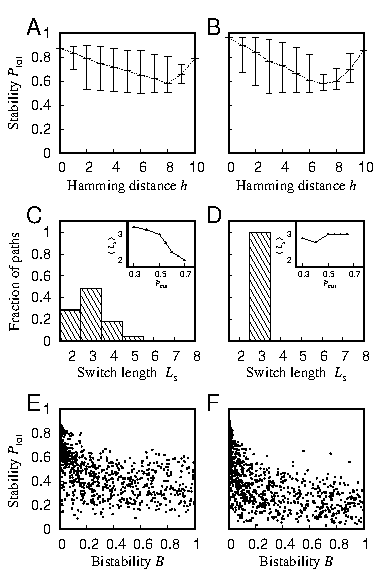
\includegraphics[width=7.8cm]{Paths}
\caption{Averages stability as a function of Hamming distance $h$. }
\end{figure}

%The smooth average stability trends in Fig.~6 might have been underpinned by individual mutational pathways that gradually shift the population between the two folds, however, this is not the case.

However, the smooth stability trends in Fig.~6A and B belie the real character of the \textit{individual} mutational pathways which tend to exhibit an abrupt switch between the two folds. To examine the statistics of fold transitions in our model, we first make a distinction between two types of stable sequences: those that fold into a single unique fold, thus behaving as classical proteins, and those that exhibit significant stabilities of both folds. Such ``bistable" sequences are interesting from a biophysical perspective in that they alternate between populating two different folds and hence are highly dynamic proteins. Indeed, they have been proposed to play an important role in the evolution of new protein folds.~\cite{Sikosek2016} 

We consider a stable sequence to be bistable if $B>0.5$, where $B$ is a bistability measure (see Fig.~6 legend); otherwise, it is considered a classical protein. In principle, a fold transition can occur directly between two classical proteins with unique folds, or it can proceed via one or more intermediate bistable sequences which populate both folds to some extent. We  define the switch length of a mutational pathway $L_\mathrm{s}=2+n_\mathrm{B}$, where $n_\mathrm{B}$ is the number of bistable sequences in between the two classical sequences that define the switch point. Hence, a path with $L_\mathrm{s}=2$ accomplishes a fold switch in a single mutational step without going through a bistable point. From the distributions of  $L_\mathrm{s}$ in Fig.~5C and D taken over all pathways with $\Pcut=0.50$, it can be seen that fold switching along individual pathways are typically completed in 1-2 mutations and often in a single step in the A1-N1 system. Hence, fold switching is typically abrupt in our model and, for $\Pcut = 0.5$, it is fairly common that viable pathways pass through one or two bistable sequences. 

Interestingly, fold switching through bistable sequences become less common as selection for more stable pathways is made in the A1-N1 system, as can be from the decrease in $\left <L_\mathrm{s}\right >$ as a function of $\Pcut$ (see Fig.~5C(inset)). For $\Pcut=0.70$, there are no longer any viable pathways between the $\alpha$-helix and $\beta$-hairpin folds that passes through a bistable point because $\left <L_\mathrm{s}\right > =  2$. The situation for the A2-TN system is different, where $\left <L_\mathrm{s}\right >$ is relatively stable around 3. For this system, there are no direct $L_\mathrm{s}=2$ paths available even at $\Pcut=0.50$. Therefore, bistable sequence play a crucial role in bridging the folds IIA and IIB even through their stabilities are significantly reduced. 

An underlying reason for the preferential behavior is apparent by comparing the total stability and bistability of all sequences. As shown in Fig.~5E and F, there is a clear trend that sequences with high total stability do not exhibit high bistability but instead they tend to have one clearly dominant fold.\\

%\subsection{Super-highways in sequence space}
%
%While there are a large number possible pathways (for $\Pcut<0.60$) in both systems, there are relatively few ways to pass between the two neutral nets. For $\Pcut=0.50$, we find that there are 109 nodes in the IA neutral net and 34 nodes in the IIB neutral net through which all viable pathways pass. For $\Pcut=0.60$, these numbers reduce to 14 and 10 nodes in the IA and IIA neutral nets, respectively.
%
 
\section{Discussion}
\noindent
We have tested a generalized-ensemble algorithm for coarse-grained simulations of biomolecules that works by making the sequence a dynamic parameter, thereby leading to a random walk in sequence space. This approach was evaluated for protein folding simulations by comparing with ST. The results indicate two main benefits of the MS approach. On the one hand, it provides a convenient way to sample the respective canonical distributions for a large set of sequences in a single run and, on the other, it also enhances the sampling of conformational space. 

The conformational sampling efficiency of the MS algorithm can be assessed from the comparison with ST in Figure~3. Although there is no single ``fair" way to compare MS and ST, we chose as a measure of efficiency the estimated statistical error on the total energy, $\sigE$, obtained with roughly the same computational cost per temperature and sequence. At the highest studied temperatures, which are well above the folding temperatures of both A1 and N1, the statistical errors $\sigE$ are basically the same for the two methods. This is not unexpected because conformational sampling of short polymers at high $T$ does not involve crossing any major energy barriers. As a result, successively sampled conformations for a given combination of sequence $\sbar$ and temperature $T$, are therefore likely mostly uncorrelated in both methods leading to similar $\sigE$ values. 

At lower temperatures, we find that the MS simulations often yields significantly smaller $\sigE$ than ST simulations. It is notable that this acceleration in conformational sampling vis-{\'a}-vis ST is achieved despite that simulations are carried out at constant temperature. Hence, rather than promoting escape from local minima in the free energy landscape by visits to higher temperature, as is the case in  ST~\cite{Marinari1992,Lyubartsev1992} or replica-exchange,~\cite{Swendsen1986}  MS simulations escape local minima through visits to sequences for which the minima may not be as deep or are altogether absent. For the same reason, the performance of the MS algorithm will depend on the size and character of sequences included. In particular, the MS simulation likely hinge on the inclusion of at least some sequences with poor stabilities such that at least partial unfolding of the chain is regularly triggered and promoting transitions to new conformational states. 

The MS method should not be seen as a general method to speed up conformational sampling due to the complexity of performing sequence updates in most biomolecular models. However, our results indicate that for coarse-grained models that permit the sequence updates as a Metropolis step and when visits to higher $T$ is unwanted (or unnecessary), the MS method can be highly efficient. A notable feature of the algorithm is that it provides escape from local minima on the free energy landscape of proteins without resorting to a change in $T$. This feature could make it attractive as an alternative to exploring the equilibrium behavior of proteins and peptides in the context or ordered dense phases such as lipid bilayers, where escape from local minima are especially challenging even in CG simulations.~\cite{Bereau2015} Simulations of lipid bilayers at elevated $T$ must typically be avoided because it can lead to unwanted perturbations of the membrane structure, although it can be a viable approach to speed up conformational sampling in particular cases.~\cite{Ulmschneider2010} 

%Overall our results show that, when technically feasible, a multisequence approach can be highly efficient for calculating the thermodynamics of a large number of amino acid sequences even at low temperatures. To demonstrate that the method to large sequence sets we applied it to the full binary sequences spaces between the model sequence pairs A1-N1 and A2-TN, which both include 1,024 sequences. These calculations would have been difficult to carry out ``in series" using some other standard method such as simulated tempering. 

%Hence, we conclude that the computational efficiency of the MS algorithm is comparable to ST. However, that while the ST simulation requires that the thermodynamic behavior is calculated at a range of temperatures, MS works well on its own directly at low temperatures. ST was introduced as an extension to the standard, fixed-$T$ Metropolis-Hastings algorithm in order to overcome the poor mixing of states at low temperatures, i.e., the tendency for the simulations at low $T$ to become trapped in local free energy minima. The MS algorithm, however, efficiently calculates the thermodynamics at low $T$'s without visits to other $T$'s. In the MS algorithm, it is visits to sequences with poor native state stability rather than high $T$'s that drive the decorrelation of generated states and escape from local traps. This way, calculation of low-$T$ thermodynamics is enhanced in MS simulations while at the same time enhancing coverage in sequence space. This makes the MS algorithm ideal for situations in which the finite-$T$ thermodynamic behavior of multiple sequences are of interest. 

%A notable feature of the MS algorithm is that provides escape from local energy minima on the free energy landscape of proteins without resorting to a change in temperature. This feature could make it attractive as an alternative to exploring the equilibrium behavior of proteins and peptides in lipid membranes, where escape from local minima are especially challenging even in CG simulations.~\cite{Bereau2015} Sampling in membrane simulations at high $T$, such as in replica-exchange simulations, are usually avoided in membrane simulations because it can lead to unwanted perturbation of the lipid bilayer structure although it can be a viable approach in particular cases.~\cite{Ulmschneider2010} 




\section{Conclusion}
\noindent
We have evaluated an algorithm for coarse-grained biomolecular simulations that allow the thermodynamics of multiple different sequences to be calculated in a single run. Here we showed that with this MS algorithm, the folding thermodynamics of over 1,000 amino acid sequences with each 35 amino acid could be determined in a coarse-grained model with 3 amino acid types. In addition to being a convenient for calculations of multiple sequences, the method enhances conformational sampling with an efficiency comparable to simulated tempering. Random walks across sequence space allow both sampling of many sequences and efficient escape from local free energy minima in the free energy landscape. The method might be well suited for coarse-grained simulations of other biomolecular systems, such as phospholipid bilayers. 

\bibliography{/Users/stefan/Documents/Manuscripts/Jshort,/Users/stefan/Documents/Manuscripts/MyRefs}

\end{document}
